\documentclass[10pt,a4paper]{article}
\author{Elijah Andrews}
\usepackage[latin1]{inputenc}
\usepackage{amsmath}
\usepackage{amsfonts}
\usepackage{amssymb}
\usepackage[labelfont=bf]{caption}
\usepackage{graphicx}
\usepackage{csvsimple}
\usepackage[left=2cm,right=2cm,top=2cm,bottom=2cm]{geometry}
\usepackage{fancyhdr}
 
\pagestyle{fancy}
\fancyhf{}
\fancyhead[LE,RO]{Elijah Andrews}
\fancyhead[RE,LO]{Aerothermodynamics Coursework}
\fancyfoot[CE,CO]{\leftmark}
\fancyfoot[LE,RO]{\thepage}

\makeatletter
\csvset{
  autotabularcenter/.style={
    file=#1,
    after head=\csv@pretable\begin{tabular}{|*{\csv@columncount}{c|}}\csv@tablehead,
    table head=\hline\csvlinetotablerow\\\hline,
    late after line=\\,
    table foot=\\\hline,
    late after last line=\csv@tablefoot\end{tabular}\csv@posttable,
    command=\csvlinetotablerow},
  autobooktabularcenter/.style={
    file=#1,
    after head=\csv@pretable\begin{tabular}{*{\csv@columncount}{c}}\csv@tablehead,
    table head=\toprule\csvlinetotablerow\\\midrule,
    late after line=\\,
    table foot=\\\bottomrule,
    late after last line=\csv@tablefoot\end{tabular}\csv@posttable,
    command=\csvlinetotablerow},
}
\makeatother
\newcommand{\csvautotabularcenter}[2][]{\csvloop{autotabularcenter={#2},#1}}
\newcommand{\csvautobooktabularcenter}[2][]{\csvloop{autobooktabularcenter={#2},#1}}

\usepackage{siunitx,array,booktabs}
\begin{document}
\section{Method of Characteristics}
The Method of Characteristics is a numerical technique used to solve partial differential equations. When applied to two-dimensional supersonic flow, assuming that it is steady and inviscid, it allows us to solve the governing compatibility equations numerically.
\\The Method of Characteristics uses characteristic lines in the flow to propagate the solution downstream. The characteristic lines are the Mach waves in supersonic flow. There are an infinite number of characteristic lines in the flow and so, starting from given flow conditions, characteristic lines can be chosen that can be used to solve a certain problem. Specific functions are constant along characteristic lines, these are known as the Riemann invariants.
For each point there are two characteristic lines, $C^{+}$ and $C^{-}$. Each of these lines has a Riemann invariant that must be constant for all points on that line. For $C^{+}$ lines, the Riemann invariant $R^{+} = \nu - \theta$. For $C^{-}$ lines, the Riemann invariant $R^{-} = \nu + \theta$.
\\Initially, points are chosen and their characteristic lines calculated. The important values that need to be calculated for the points are the Prandtl-Meyer function $\nu(M)$, flow angle $\theta$, and Mach angle $\mu$. These can be obtained from known conditions and used to calculate the Riemann invariants for that point. The characteristic lines from that point can then be traced downstream. This process is repeated for multiple initial points.
\\Where two characteristic lines cross a new point can be defined and its values for $\nu$ and $\theta$ calculated. These can then be used to determine the Mach number (usually using an isentropic flow table), Mach angle, and hence point coordinates.
\\When considering symmetric flows, such as that in a 2D symmetric nozzle, a centreline can be defined about which the solution is also symmetric. This property can be used to reduce the number of points that need to be calculated by half. For a point along the line of symmetry, the incoming $C^{-}$ is assumed to be the same as an incoming $C^{+}$ from the opposite side, and thus the $R^{-}$ and $R^{+}$ values for the point would be equal.
\\Using these calculations, the solution can be marched downstream and the values obtained can be used to determine properties of the flow as with other methods of flow simulation.
\\Of particular interest is the case where the Method of Characteristics can be used to determine the shortest length that a supersonic nozzle can be to have perfectly expanded flow in specified conditions. In this case the initial points are all at the wall of the throat and have different characteristic lines starting from small angles and increasing up to $\theta_{max} = \nu (M) / 2$. The flow is solved as above. Once a characteristic line has been 'reflected' by the line of symmetry it then passes through all of the characteristic lines $C^{-}$ from the subsequent initial points and then impinges on the nozzle wall. The 'reflected' characteristic line is used as $C^{+}$ and the previous point along the wall is used as $C^{-}$. The coordinates calculated for these wall points can be used to determine the nozzle contour and hence the minimum length of the nozzle.
\section{Tables}
\begin{center}
\begin{large}
\textbf{Lookup Table} ($\gamma=5/3$)
\end{large}
\\\csvautobooktabularcenter[table head=\toprule\bfseries M & \bfseries $\mu$ (deg.) & \bfseries $\nu$ (deg.)\\\midrule\csvlinetotablerow\\, before reading=\centering]{argon_ift.csv}
\end{center}

\begin{center}
\begin{large}
\textbf{Method of Characteristics Table} ($\gamma=5/3$, $M_{des}=2.4$)
\end{large}
\\\textit{Linear interpolation between values in the lookup table has been used to improve the accuracy of results.}
\csvautobooktabularcenter[table head=\toprule\bfseries Point & \bfseries $\mathbf{R^{+}}$ & \bfseries $\mathbf{R^{-}}$ & \bfseries $\mathbf{\theta}$ & \bfseries $\mathbf{\nu}$ & \bfseries M & \bfseries $\mathbf{\mu}$ & \bfseries $\mathbf{\theta + \mu}$ & \bfseries $\mathbf{\theta - \mu}$ & \bfseries x & \bfseries y\\\midrule\csvlinetotablerow\\, before reading=\centering]{MoC.csv}
\end{center}
\section{Results}
The results above can be compared to quasi 1D theory. Quasi 1D theory shows that the area ratio between the nozzle exit area and the nozzle throat area is a function of the exit Mach number and $\gamma$ when assuming the flow acts in one dimension only. For our values of $\gamma = 5/3$ and design Mach number $M_{des}=2.4$, quasi 1D theory shows that the area ratio should be 1.998. Since we are using a 2D nozzle, the area ratio is equivalent to the ratio of heights between the nozzle exit and the nozzle throat. In the Method of Characteristics table the height of the nozzle exit is calculated to be 1.995, since the nozzle throat has a height of 1 this is equivalent to the area ratio.
\\The calculated value, 1.995, is close to the theoretical quasi 1D value, 1.998, as shown in figure \ref{fig:nozzle_profile}, which suggests that the Method of Characteristics result is valid. However, there is a difference due to the assumptions that are made for each method.
\\Quasi 1D theory assumes that the velocity is primarily in the x direction, whereas the Method of Characteristics accounts for 2D flow directions. 
\\For the Method of Characteristics, error is added by assuming that the flow is irrotational so that we can apply isentropic relations to the assumed homentropic flow using Crocco's theorem.
\\The Method of Characteristics is discontinuous whereas quasi 1D theory is an integral solution and so is continuous. Due to the discontinuous nature of the Method of Characteristics, a lot of error is added through the iteration of the solution as error between points is compounded and the assumption that the flow acts predictably between points may be incorrect. This can be improved by increasing the number of initial points used so that the distance between points is reduced. Figure \ref{fig:y_coordinates} shows that as the number of initial points increases, the final y coordinate of the nozzle tends towards some value. It shows that for a more accurate solution, a minimum of 40 initial points should be used as this is beyond the initial instability of the results.
\\In addition to these, error is added by using the Lookup Table above rather than more precise solutions. Linear interpolation between values has been used to generate the Method of Characteristics Table to improve accuracy. However, this still introduces additional error to the solution. Better interpolation techniques, a higher resolution lookup table, or a high precision numerical solution to the equations that generate the lookup table could all reduce this error, possibly at the cost of computation speed.
\begin{figure}[!htb]
\centering
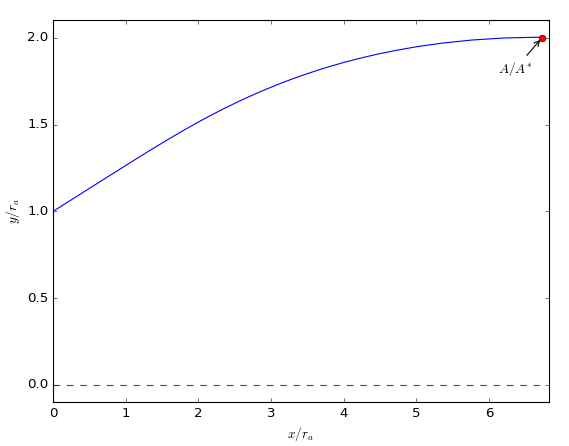
\includegraphics[scale=0.75]{nozzle.png}
\caption{A graph showing the nozzle profile and equivalent $A/A^{*}$ value.}
\label{fig:nozzle_profile}
\end{figure}
\begin{figure}[!htb]
\centering
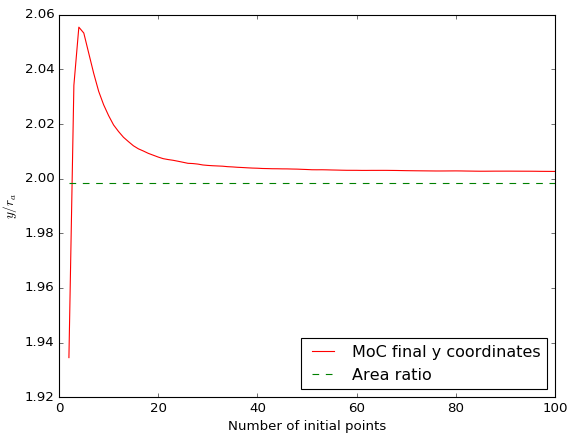
\includegraphics[scale=0.75]{accuracy.png}
\caption{A graph showing the final wall point y value against the number of initial points used and the $A/A^{*}$ value.}
\label{fig:y_coordinates}
\end{figure}
\end{document}
